\begin{frame}[fragile]{Análisis de MainActivity\_Demo19}
\textbf{Clase: MainActivity\_Demo19}

\begin{itemize}
    \item Es la actividad principal de una aplicación Android.
    \item Extiende de \texttt{AppCompatActivity}.
    \item Se encarga de inicializar la interfaz y la vista del juego Pong (\textbf{PongSurfaceView:}).
\end{itemize}


\begin{itemize}
    \item En \texttt{onCreate()}:
    \begin{itemize}
        \item Se obtiene la referencia a \texttt{PongSurfaceView} con \texttt{findViewById()}.
		\item \textbf{Ciclo de vida:}
		\begin{itemize}
			\item \texttt{onResume()} y \texttt{onPause()} están definidos pero sin lógica adicional.
			\item Normalmente se usarían para pausar/reanudar el hilo del juego.
		\end{itemize}
    \end{itemize}
\end{itemize}

\textbf{Idea clave:}
\begin{itemize}
    \item La Activity actúa como contenedor, mientras que toda la lógica y renderizado del juego ocurre en \texttt{PongSurfaceView}.
\end{itemize}

\end{frame}


\begin{frame}[fragile]{Game Loop en PongSurfaceView (Android)}
\textbf{¿Qué es el Game Loop?}

\begin{itemize}
    \item Es un ciclo continuo que controla la ejecución de un videojuego.
    \item Se encarga de:
    \begin{itemize}
        \item Actualizar la lógica del juego.
        \item Dibujar los elementos en pantalla.
        \item Controlar la velocidad (FPS).
    \end{itemize}
\end{itemize}

\textbf{Implementación en SurfaceView:}
\begin{itemize}
    \item Se ejecuta en un hilo independiente del UI thread.
    \item Usa \textbf{SurfaceHolder} para dibujar sobre el \textbf{Canvas}.
\end{itemize}


\textbf{Métodos clave:}
\begin{itemize}
    \item \textbf{update():} Movimiento de pelota, colisiones, puntaje.
    \item \textbf{draw():} Dibujo en Canvas (paletas, pelota, fondo).
    \item \textbf{controlFPS():} Regula la velocidad del juego.
\end{itemize}


\textbf{Idea clave:}
\begin{itemize}
    \item El Game Loop permite animaciones fluidas y control total del juego en tiempo real.
\end{itemize}

\end{frame}



\begin{frame}[fragile]
\frametitle{Demo 19: Pong Game }
\begin{columns}
\column{0.80\linewidth}

\scriptsize
Del Repositorio Github:
\begin{itemize}
%\item Agregar la siguiente linea: \textit{implementation("com.github.PhilJay:MPAndroidChart:v3.1.0")}, al final de la seccion Dependencies del archivo Build.graddle.kts (Module: App).
%\item Agregar la siguiente linea: \textit{maven \{ url = uri(``https://jitpack.io'') \}}, al final de la seccion \textit{dependencyResolutionManagement } del archivo settings.graddle.kts.
\item Copiar el archivo \textit{MainActivity\_Demo19.java} (dentro del Folder códigosJAVA) al mismo directorio donde esta el MainActivity.java
\item Copiar los archivos \textit{TicTacToeView.java},  (dentro del Folder códigosJAVA) al mismo directorio donde esta el MainActivity.java
\item Copiar el archivo \textit{activity\_main\_demo19.xml} (dentro del Folder Carpeta\_layout) al mismo directorio donde esta el activity\_main.xml
\item Modificar dentro del archivo \textit{activity\_main\_demo19.xml} la cadena \textit{.com.example.a2026\_01\_holamundoandroid.PongSurfaceView} por \textit{$<$SuPackage$>$.PongSurfaceView}.
\item Modificar en el archivo \textit{AndroidManifest.xml} la cadena \textit{.MainActivity\_Demo18} por \textit{.MainActivity\_Demo19}.


%\item Ir a la linea 22 de archivo del archivo \textit{MainActivity\_Demo09.java}, poner el cursos en la palabra (en Rojo) \textit{documentfile}, presionar la combinación ALT+ENTER, y seleccionar de la lista desplegable la opcion ``Add dependency on ....''. Esto quitará el error y hara los ajustes necesarios. 
\end{itemize}

%\begin{block}{Demo \#09}
%Un App que permite escribir el contenido de un EditText a un archivo y cargar el contenido de cualquier archivo en el EditText
%\end{block}


\column{0.20\linewidth}

\begin{center}
 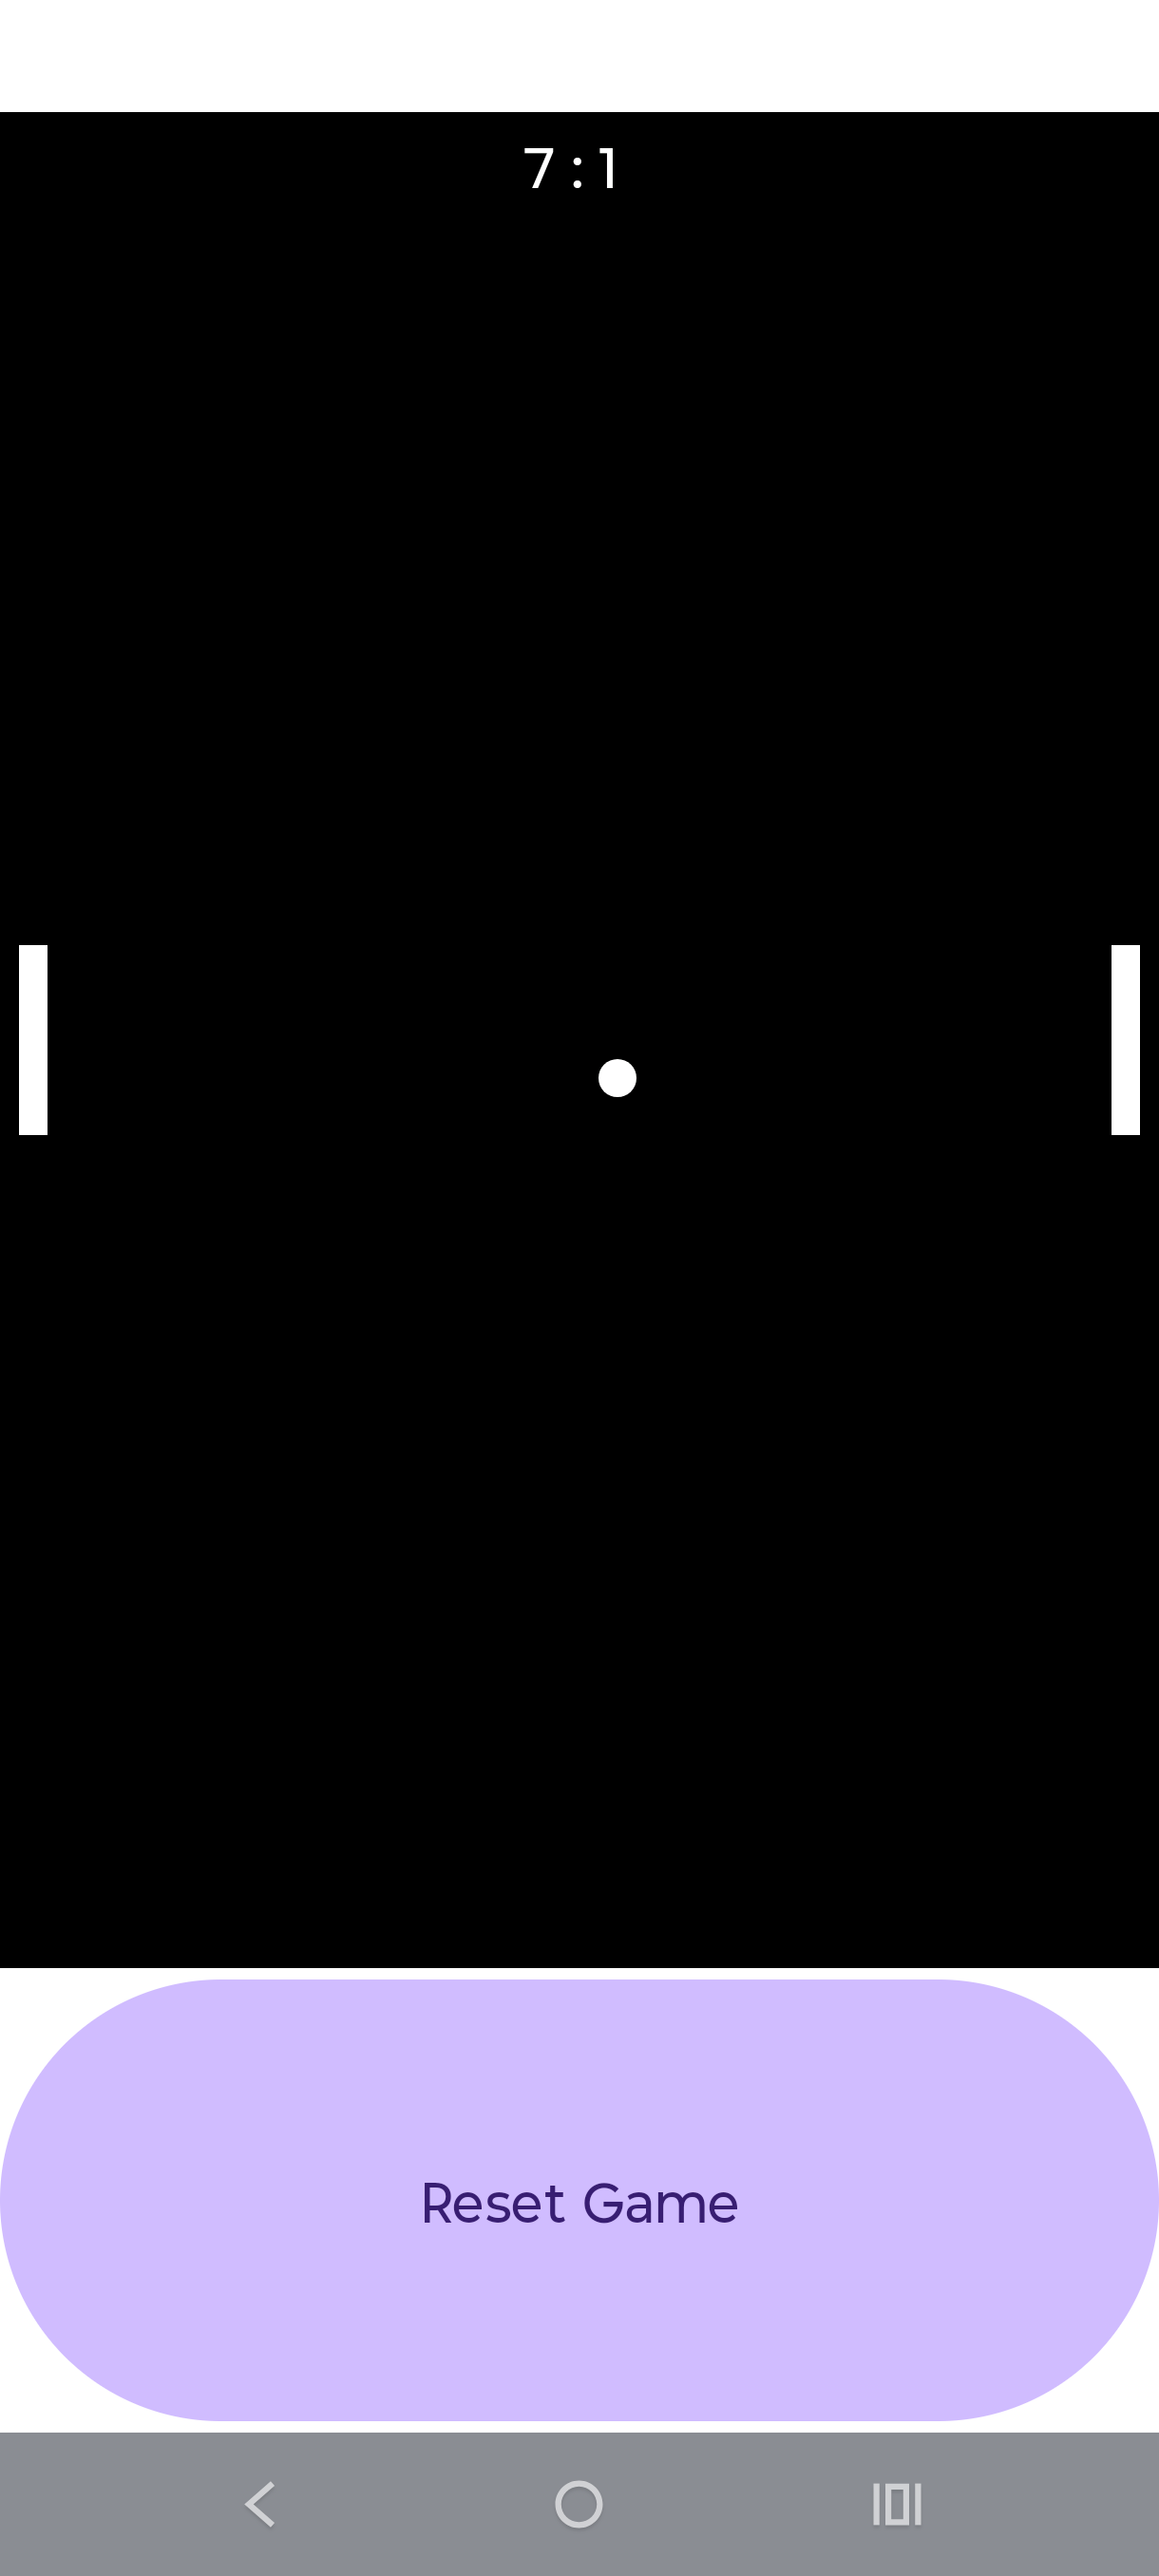
\includegraphics[width=0.98\textwidth]{02_TallerCBTis/figs/Demo19}
\end{center}

\end{columns}

\end{frame}

